\documentclass[twoside]{book}

% Packages required by doxygen
\usepackage{calc}
\usepackage{doxygen}
\usepackage{graphicx}
\usepackage[utf8]{inputenc}
\usepackage{makeidx}
\usepackage{multicol}
\usepackage{multirow}
\usepackage{textcomp}
\usepackage[table]{xcolor}

% Font selection
\usepackage[T1]{fontenc}
\usepackage{mathptmx}
\usepackage[scaled=.90]{helvet}
\usepackage{courier}
\usepackage{amssymb}
\usepackage{sectsty}
\renewcommand{\familydefault}{\sfdefault}
\allsectionsfont{%
  \fontseries{bc}\selectfont%
  \color{darkgray}%
}
\renewcommand{\DoxyLabelFont}{%
  \fontseries{bc}\selectfont%
  \color{darkgray}%
}

% Page & text layout
\usepackage{geometry}
\geometry{%
  a4paper,%
  top=2.5cm,%
  bottom=2.5cm,%
  left=2.5cm,%
  right=2.5cm%
}
\tolerance=750
\hfuzz=15pt
\hbadness=750
\setlength{\emergencystretch}{15pt}
\setlength{\parindent}{0cm}
\setlength{\parskip}{0.2cm}
\makeatletter
\renewcommand{\paragraph}{%
  \@startsection{paragraph}{4}{0ex}{-1.0ex}{1.0ex}{%
    \normalfont\normalsize\bfseries\SS@parafont%
  }%
}
\renewcommand{\subparagraph}{%
  \@startsection{subparagraph}{5}{0ex}{-1.0ex}{1.0ex}{%
    \normalfont\normalsize\bfseries\SS@subparafont%
  }%
}
\makeatother

% Headers & footers
\usepackage{fancyhdr}
\pagestyle{fancyplain}
\fancyhead[LE]{\fancyplain{}{\bfseries\thepage}}
\fancyhead[CE]{\fancyplain{}{}}
\fancyhead[RE]{\fancyplain{}{\bfseries\leftmark}}
\fancyhead[LO]{\fancyplain{}{\bfseries\rightmark}}
\fancyhead[CO]{\fancyplain{}{}}
\fancyhead[RO]{\fancyplain{}{\bfseries\thepage}}
\fancyfoot[LE]{\fancyplain{}{}}
\fancyfoot[CE]{\fancyplain{}{}}
\fancyfoot[RE]{\fancyplain{}{\bfseries\scriptsize Generated on Mon May 15 2017 21\-:15\-:16 for My Project by Doxygen }}
\fancyfoot[LO]{\fancyplain{}{\bfseries\scriptsize Generated on Mon May 15 2017 21\-:15\-:16 for My Project by Doxygen }}
\fancyfoot[CO]{\fancyplain{}{}}
\fancyfoot[RO]{\fancyplain{}{}}
\renewcommand{\footrulewidth}{0.4pt}
\renewcommand{\chaptermark}[1]{%
  \markboth{#1}{}%
}
\renewcommand{\sectionmark}[1]{%
  \markright{\thesection\ #1}%
}

% Indices & bibliography
\usepackage{natbib}
\usepackage[titles]{tocloft}
\setcounter{tocdepth}{3}
\setcounter{secnumdepth}{5}
\makeindex

% Hyperlinks (required, but should be loaded last)
\usepackage{ifpdf}
\ifpdf
  \usepackage[pdftex,pagebackref=true]{hyperref}
\else
  \usepackage[ps2pdf,pagebackref=true]{hyperref}
\fi
\hypersetup{%
  colorlinks=true,%
  linkcolor=blue,%
  citecolor=blue,%
  unicode%
}

% Custom commands
\newcommand{\clearemptydoublepage}{%
  \newpage{\pagestyle{empty}\cleardoublepage}%
}


%===== C O N T E N T S =====

\begin{document}

% Titlepage & ToC
\hypersetup{pageanchor=false}
\pagenumbering{roman}
\begin{titlepage}
\vspace*{7cm}
\begin{center}%
{\Large My Project }\\
\vspace*{1cm}
{\large Generated by Doxygen 1.8.6}\\
\vspace*{0.5cm}
{\small Mon May 15 2017 21:15:16}\\
\end{center}
\end{titlepage}
\clearemptydoublepage
\tableofcontents
\clearemptydoublepage
\pagenumbering{arabic}
\hypersetup{pageanchor=true}

%--- Begin generated contents ---
\chapter{Hierarchical Index}
\section{Class Hierarchy}
This inheritance list is sorted roughly, but not completely, alphabetically\+:\begin{DoxyCompactList}
\item \contentsline{section}{twitter.\+views.\+Twitter\+Stats}{\pageref{classtwitter_1_1views_1_1_twitter_stats}}{}
\item App\+Config\begin{DoxyCompactList}
\item \contentsline{section}{twitter.\+apps.\+Twitter\+Config}{\pageref{classtwitter_1_1apps_1_1_twitter_config}}{}
\end{DoxyCompactList}
\item Test\+Case\begin{DoxyCompactList}
\item \contentsline{section}{twitter.\+tests.\+Stats\+Test\+Cases}{\pageref{classtwitter_1_1tests_1_1_stats_test_cases}}{}
\end{DoxyCompactList}
\end{DoxyCompactList}

\chapter{Class Index}
\section{Class List}
Here are the classes, structs, unions and interfaces with brief descriptions\+:\begin{DoxyCompactList}
\item\contentsline{section}{\hyperlink{classtwitter_1_1tests_1_1_stats_test_cases}{twitter.\+tests.\+Stats\+Test\+Cases} }{\pageref{classtwitter_1_1tests_1_1_stats_test_cases}}{}
\item\contentsline{section}{\hyperlink{classtwitter_1_1apps_1_1_twitter_config}{twitter.\+apps.\+Twitter\+Config} }{\pageref{classtwitter_1_1apps_1_1_twitter_config}}{}
\item\contentsline{section}{\hyperlink{classtwitter_1_1views_1_1_twitter_stats}{twitter.\+views.\+Twitter\+Stats} }{\pageref{classtwitter_1_1views_1_1_twitter_stats}}{}
\end{DoxyCompactList}

\chapter{Class Documentation}
\hypertarget{classtwitter_1_1tests_1_1StatsTestCases}{\section{twitter.\-tests.\-Stats\-Test\-Cases Class Reference}
\label{classtwitter_1_1tests_1_1StatsTestCases}\index{twitter.\-tests.\-Stats\-Test\-Cases@{twitter.\-tests.\-Stats\-Test\-Cases}}
}
Inheritance diagram for twitter.\-tests.\-Stats\-Test\-Cases\-:\begin{figure}[H]
\begin{center}
\leavevmode
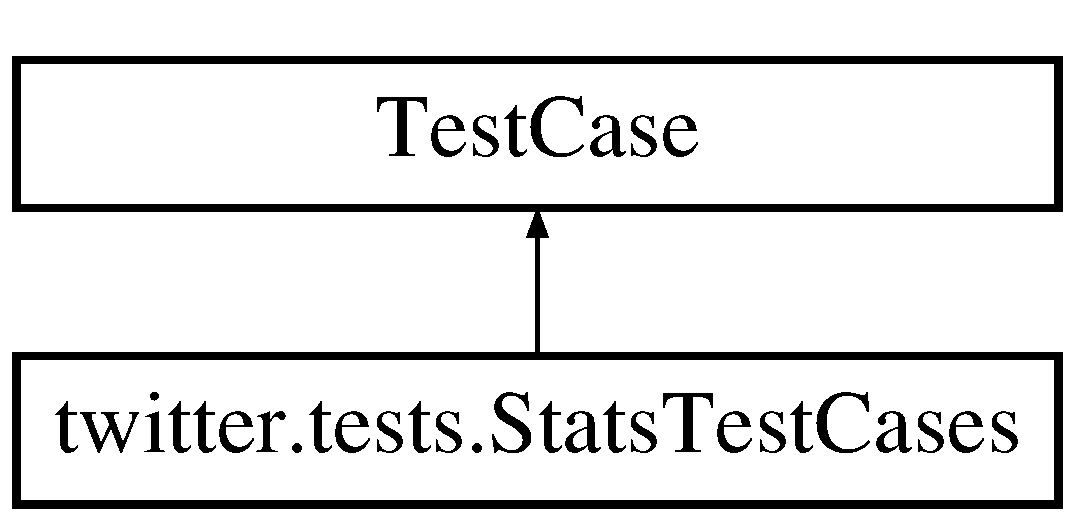
\includegraphics[height=2.000000cm]{classtwitter_1_1tests_1_1StatsTestCases}
\end{center}
\end{figure}
\subsection*{Public Member Functions}
\begin{DoxyCompactItemize}
\item 
\hypertarget{classtwitter_1_1tests_1_1StatsTestCases_a924d247a4518455ba5ad682e9e7f95b4}{def {\bfseries test\-\_\-get\-Frequency\-Of\-Words\-Of\-Liked\-Tweets}}\label{classtwitter_1_1tests_1_1StatsTestCases_a924d247a4518455ba5ad682e9e7f95b4}

\item 
\hypertarget{classtwitter_1_1tests_1_1StatsTestCases_abdf69a763661d75a0abcd8d02182204d}{def {\bfseries test\-\_\-get\-Most\-Liked\-Pages}}\label{classtwitter_1_1tests_1_1StatsTestCases_abdf69a763661d75a0abcd8d02182204d}

\item 
\hypertarget{classtwitter_1_1tests_1_1StatsTestCases_ac9bc89051719ae99de701333f1cad0a2}{def {\bfseries test\-\_\-get\-Users\-Tweeting\-Most\-Frequently}}\label{classtwitter_1_1tests_1_1StatsTestCases_ac9bc89051719ae99de701333f1cad0a2}

\item 
\hypertarget{classtwitter_1_1tests_1_1StatsTestCases_ac284bee5f974f70566ad7994ce85d6db}{def {\bfseries test\-\_\-get\-Frequency\-Of\-Words\-Of\-All\-Tweets}}\label{classtwitter_1_1tests_1_1StatsTestCases_ac284bee5f974f70566ad7994ce85d6db}

\item 
\hypertarget{classtwitter_1_1tests_1_1StatsTestCases_aa0c7de435227ee6b49566f4cebe41801}{def {\bfseries test\-\_\-get\-Like\-Ratio\-Of\-Two\-Users}}\label{classtwitter_1_1tests_1_1StatsTestCases_aa0c7de435227ee6b49566f4cebe41801}

\item 
\hypertarget{classtwitter_1_1tests_1_1StatsTestCases_afeb0ed8b27ae13e5a15dc722da42c0e8}{def {\bfseries test\-\_\-get\-Hashtag\-Percentage}}\label{classtwitter_1_1tests_1_1StatsTestCases_afeb0ed8b27ae13e5a15dc722da42c0e8}

\item 
\hypertarget{classtwitter_1_1tests_1_1StatsTestCases_a8402cdedfe664593cbffff181f066b99}{def {\bfseries test\-\_\-get\-Most\-Number\-Of\-Followers}}\label{classtwitter_1_1tests_1_1StatsTestCases_a8402cdedfe664593cbffff181f066b99}

\end{DoxyCompactItemize}


The documentation for this class was generated from the following file\-:\begin{DoxyCompactItemize}
\item 
tests.\-py\end{DoxyCompactItemize}

\hypertarget{classtwitter_1_1apps_1_1TwitterConfig}{\section{twitter.\-apps.\-Twitter\-Config Class Reference}
\label{classtwitter_1_1apps_1_1TwitterConfig}\index{twitter.\-apps.\-Twitter\-Config@{twitter.\-apps.\-Twitter\-Config}}
}
Inheritance diagram for twitter.\-apps.\-Twitter\-Config\-:\begin{figure}[H]
\begin{center}
\leavevmode
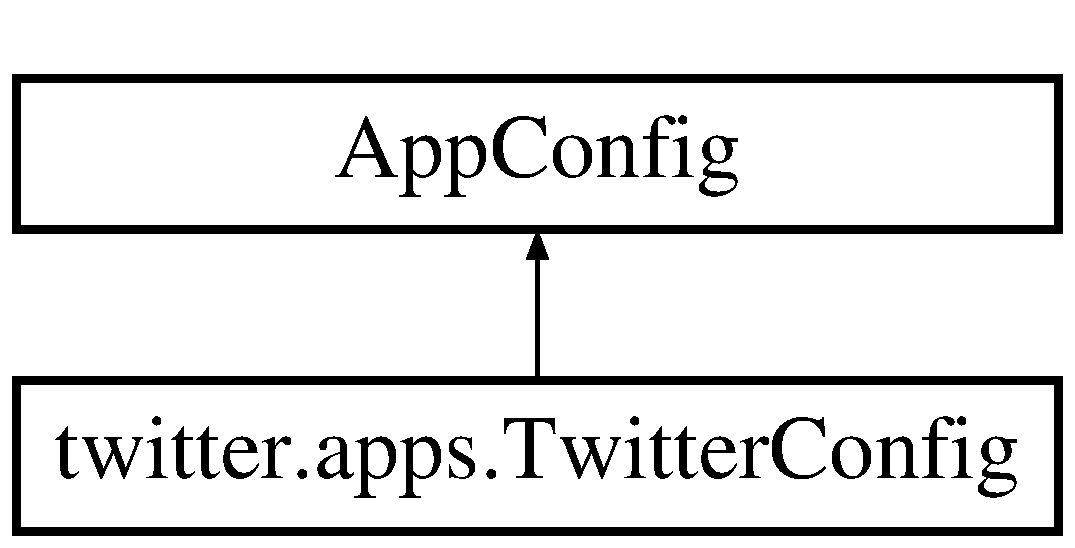
\includegraphics[height=2.000000cm]{classtwitter_1_1apps_1_1TwitterConfig}
\end{center}
\end{figure}
\subsection*{Static Public Attributes}
\begin{DoxyCompactItemize}
\item 
\hypertarget{classtwitter_1_1apps_1_1TwitterConfig_ad6fa8da3b1d7a28a13a3a1430d9ad93f}{string {\bfseries name} = 'twitter'}\label{classtwitter_1_1apps_1_1TwitterConfig_ad6fa8da3b1d7a28a13a3a1430d9ad93f}

\end{DoxyCompactItemize}


The documentation for this class was generated from the following file\-:\begin{DoxyCompactItemize}
\item 
apps.\-py\end{DoxyCompactItemize}

\hypertarget{classtwitter_1_1views_1_1TwitterStats}{\section{twitter.\-views.\-Twitter\-Stats Class Reference}
\label{classtwitter_1_1views_1_1TwitterStats}\index{twitter.\-views.\-Twitter\-Stats@{twitter.\-views.\-Twitter\-Stats}}
}
\subsection*{Public Member Functions}
\begin{DoxyCompactItemize}
\item 
\hypertarget{classtwitter_1_1views_1_1TwitterStats_a4ed5b049b9cc36bd7bc561399586530a}{def {\bfseries index}}\label{classtwitter_1_1views_1_1TwitterStats_a4ed5b049b9cc36bd7bc561399586530a}

\item 
\hypertarget{classtwitter_1_1views_1_1TwitterStats_a04c9399fea71d988f011da7cbbc52f2e}{def {\bfseries example}}\label{classtwitter_1_1views_1_1TwitterStats_a04c9399fea71d988f011da7cbbc52f2e}

\item 
\hypertarget{classtwitter_1_1views_1_1TwitterStats_ac25d6a140308ebb4e3ac36fe77dfb05b}{def {\bfseries get\-Users\-Tweeting\-Most\-Frequently}}\label{classtwitter_1_1views_1_1TwitterStats_ac25d6a140308ebb4e3ac36fe77dfb05b}

\item 
def \hyperlink{classtwitter_1_1views_1_1TwitterStats_a6ca5eaaaea6d0cc6f3ba6adf1e43a77a}{get\-Frequency\-Of\-Words\-Of\-Liked\-Tweets}
\item 
\hypertarget{classtwitter_1_1views_1_1TwitterStats_ac3d5509bd20a5236580825fe9d729288}{def {\bfseries get\-Most\-Number\-Of\-Followers}}\label{classtwitter_1_1views_1_1TwitterStats_ac3d5509bd20a5236580825fe9d729288}

\item 
\hypertarget{classtwitter_1_1views_1_1TwitterStats_a2bd86bb15f6a672135501f511d87a7f4}{def {\bfseries get\-Most\-Liked\-Pages}}\label{classtwitter_1_1views_1_1TwitterStats_a2bd86bb15f6a672135501f511d87a7f4}

\item 
\hypertarget{classtwitter_1_1views_1_1TwitterStats_a653aa5d8b561876322389e18566cfea1}{def {\bfseries get\-Who\-Mentioned\-Most}}\label{classtwitter_1_1views_1_1TwitterStats_a653aa5d8b561876322389e18566cfea1}

\item 
\hypertarget{classtwitter_1_1views_1_1TwitterStats_a2f62ab9591fe2de8580d32cd5e644c1a}{def {\bfseries get\-Like\-Ratio\-Of\-Two\-Users}}\label{classtwitter_1_1views_1_1TwitterStats_a2f62ab9591fe2de8580d32cd5e644c1a}

\item 
\hypertarget{classtwitter_1_1views_1_1TwitterStats_a16c9204d619bc372b5514e14b0f3f2f7}{def {\bfseries get\-Frequency\-Of\-Words\-Of\-All\-Tweets}}\label{classtwitter_1_1views_1_1TwitterStats_a16c9204d619bc372b5514e14b0f3f2f7}

\item 
\hypertarget{classtwitter_1_1views_1_1TwitterStats_ade56dd927ad6ab3c97f19df278f8c168}{def {\bfseries hashtag\-Percentage}}\label{classtwitter_1_1views_1_1TwitterStats_ade56dd927ad6ab3c97f19df278f8c168}

\end{DoxyCompactItemize}
\subsection*{Static Public Member Functions}
\begin{DoxyCompactItemize}
\item 
\hypertarget{classtwitter_1_1views_1_1TwitterStats_a8e9604d5d19a469a4dc9386cf8d29557}{def {\bfseries get\-Twitter\-Api}}\label{classtwitter_1_1views_1_1TwitterStats_a8e9604d5d19a469a4dc9386cf8d29557}

\end{DoxyCompactItemize}


\subsection{Member Function Documentation}
\hypertarget{classtwitter_1_1views_1_1TwitterStats_a6ca5eaaaea6d0cc6f3ba6adf1e43a77a}{\index{twitter\-::views\-::\-Twitter\-Stats@{twitter\-::views\-::\-Twitter\-Stats}!get\-Frequency\-Of\-Words\-Of\-Liked\-Tweets@{get\-Frequency\-Of\-Words\-Of\-Liked\-Tweets}}
\index{get\-Frequency\-Of\-Words\-Of\-Liked\-Tweets@{get\-Frequency\-Of\-Words\-Of\-Liked\-Tweets}!twitter::views::TwitterStats@{twitter\-::views\-::\-Twitter\-Stats}}
\subsubsection[{get\-Frequency\-Of\-Words\-Of\-Liked\-Tweets}]{\setlength{\rightskip}{0pt plus 5cm}def twitter.\-views.\-Twitter\-Stats.\-get\-Frequency\-Of\-Words\-Of\-Liked\-Tweets (
\begin{DoxyParamCaption}
\item[{}]{request}
\end{DoxyParamCaption}
)}}\label{classtwitter_1_1views_1_1TwitterStats_a6ca5eaaaea6d0cc6f3ba6adf1e43a77a}
\begin{DoxyVerb}This method counts the frequency of the words a specific user liked.
It has two paramters, username and count where username is compulsory.
If a username is not provided, method returns a string that expresses this fact.
If count is not provided, it is defaulted to 100, hence only 100 tweets is searched.
!@param count, username 
!@author Rıza Özçelik
\end{DoxyVerb}
 

The documentation for this class was generated from the following file\-:\begin{DoxyCompactItemize}
\item 
views.\-py\end{DoxyCompactItemize}

%--- End generated contents ---

% Index
\newpage
\phantomsection
\addcontentsline{toc}{chapter}{Index}
\printindex

\end{document}
